%\documentclass[oneside, DIV=11, BCOR=10mm]{scrbook}
\documentclass[oneside]{scrbook}
\usepackage[english]{babel}
\usepackage[T1]{fontenc}
\usepackage{amsmath}
\usepackage{booktabs}
\usepackage{mathtools}
\usepackage{graphicx}
\usepackage{xspace}
\usepackage{cite}
\usepackage{minitoc}
\setcounter{minitocdepth}{3}
\usepackage[xindy,toc]{glossaries}
\usepackage{todonotes}
\usepackage{units}
\usepackage{xstring}
\usepackage[round,colon]{natbib}
\usepackage[activate={true,nocompatibility}]{microtype}
% code listings
\usepackage{listings}
\usepackage{multicol}
\usepackage{url}
\usepackage{bytefield}
\lstdefinelanguage{powerasm}{
  morekeywords={extern,text,add,addi,b,bl,stw,lis,li,lwz,synmtvr,synmfvr,synops,synswp,synm,syncmpi,syns,wait},
  sensitive=true,
  morecomment=[l]{\#}
}
\lstset{
    basicstyle=\footnotesize\ttfamily,
    numbers=left,
    numberstyle=\tiny,
    %stepnumber=5,
    numbersep=5pt,
    tabsize=2,
    breaklines=true,
    xleftmargin=17pt,
    framexleftmargin=17pt,
    framexrightmargin=5pt,
    framexbottommargin=4pt
}
\lstloadlanguages{powerasm,c,bash}
\usepackage{algpseudocode}
% clickable links
\usepackage[
  pdftex,
  pdfauthor={Simon Friedmann},
  pdftitle={Plasticity Processor User Guide}
]{hyperref}
\hypersetup{
  hidelinks=true,
  colorlinks=false,
  urlcolor=black,
  linkcolor=black,
  citecolor=black
}
% font selection
\usepackage{mathpazo}
\usepackage[scaled]{berasans}
\usepackage{courier}

\title{Nux User Guide}
\author{Simon Friedmann}

%
% Glossaries
%
\makeglossaries
\loadglsentries{src/glossaries.tex}

%
% custom macros
%

% template to typeset identifiers from code containing _ and :: characters
\newcommand{\code}[1]{\texttt{%
    \noexpandarg %
    \StrSubstitute{#1}{_}{\textunderscore}[\x]%
    \expandafter\StrSubstitute\expandafter{\x}{::}{$\dblcolon$}[\x]%
    \x}\xspace}

% template for file references
\newcommand{\file}[1]{\path{#1}\xspace}

% template for global parameter description list
\newcommand{\ppuParameter}[4]{%
    \item[\code{#1}]
        type: \code{#2}, default: #3

        #4
}

% template for port description list items
\newcommand{\portItem}[3]{%
    \item[\code{#1}]
        type: \code{#2}

        #3}

% \fxvinst{name}{mnemnonic}{xo-code}{coding}{algorithm}{text}
\newcommand{\fxvinst}[5]{%
    \subsubsection[#2]{#1} % show mnemnonic in table of contents
    \begin{bytefield}[bitwidth=0.5\textwidth/32]{32}
        \bitheader{0,5,10,15,20,29,31} \\
        \bitbox{6}{4}  \bitbox{5}{VRT}  \bitbox{5}{VRA}  \bitbox{5}{VRB}  \bitbox{9}{#3}  \bitbox{2}{C}
    \end{bytefield} \\
    \textbf{#2}\\
    {\footnotesize
    \begin{algorithmic}[1]
    #4
    \end{algorithmic} }
    #5
}

% \fxvinstGPR{name}{mnemnonic}{xo-code}{coding}{algorithm}{text}
\newcommand{\fxvinstGPR}[5]{%
    \subsubsection[#2]{#1} % show mnemnonic in table of contents
    \begin{bytefield}[bitwidth=0.5\textwidth/32]{32}
        \bitheader{0,5,10,15,20,29,31} \\
        \bitbox{6}{4}  \bitbox{5}{VRT}  \bitbox{5}{RA}  \bitbox{5}{RB}  \bitbox{9}{#3}  \bitbox{2}{/}
    \end{bytefield} \\
    \textbf{#2}\\
    {\footnotesize
    \begin{algorithmic}[1]
        #4
    \end{algorithmic} }
    #5
}

% \fxvinstGPRa{name}{mnemnonic}{xo-code}{coding}{algorithm}{text}
\newcommand{\fxvinstGPRa}[5]{%
    \subsubsection[#2]{#1} % show mnemnonic in table of contents
    \begin{bytefield}[bitwidth=0.5\textwidth/32]{32}
        \bitheader{0,5,10,15,20,29,31} \\
        \bitbox{6}{4}  \bitbox{5}{VRT}  \bitbox{5}{RA}  \bitbox{5}{/}  \bitbox{9}{#3}  \bitbox{2}{/}
    \end{bytefield} \\
    \textbf{#2}\\
    {\footnotesize
    \begin{algorithmic}[1]
        #4
    \end{algorithmic} }
    #5
}

\begin{document}

	\maketitle
    \dominitoc
    \tableofcontents

    \chapter{Introduction}

\section{Scope of this document}
This user guide intends to give an overview of the Nux's design and how to use it in hardware designs and for executing software on it.
It is not a full specification.
It should serve as a starting point for everyone wanting to contribute to the design and provide the necessary knowledge to use it in other hardware designs.


\section{Related material}
Most of the internals are documented in detail in \cite{friedmann13phd}.
Some overview of the vector \gls{simd} unit and the use for plasticity is given in \cite{dlspaper15}.


    \chapter{Instantiating Nux}


\section{Design parameters}
The top-level module \code{Pu_v2} offers a large number of parameters that control various aspects of the design.
Additionally some important parameters are hidden deeper in the code.
This section lists and describes those parameters.

\subsection{Top-level parameters}
\label{sec:topopt}

First, the top-level design parameters (see also file \file{rtl/processor/pu.sv}):
\begin{description}
    \ppuParameter{OPT_BCACHE}{int}{0}{%
        Configures the branch predictor (branch cache).
        A value of 0 disables branch prediction completely.
        Higher values control the number of entries in the branch cache.
        The branch cache contains $2^{\text{\code{OPT_BCACHE}}}$ entries.
    }
    \ppuParameter{OPT_MULTIPLIER}{bit}{1}{%
        Set to one to include a fixed-point multiplier in the design.
    }
    \ppuParameter{OPT_DIVIDER}{bit}{1}{%
        Set to one to include a fixed-point divider in the design.
    }
    \ppuParameter{OPT_IOBUS}{bit}{1}{%
        Include an \gls{omnibus} interface for use by the external control facility (see~\cite{powerisa_206}).
        The interface is called \code{iobus}.
    }
    \ppuParameter{OPT_VECTOR}{bit}{1}{%
        Set to one to include the \gls{fxv} \gls{simd} extension.
        Enables also the \code{vector_bus} interface for serial load/store accesses (\code{fxvlax}, \code{fxvstax}) and \code{vector_pbus} for parallel load/store accesses (\code{fxvinx}, \code{fxvoutx}).
    }
    \ppuParameter{OPT_VECTOR_SLICES}{int}{8}{%
        Control the number of parallel datapath blocks called slices in the \gls{fxv} unit.
    }
    \ppuParameter{OPT_VECTOR_NUM_HALFWORDS}{int}{8}{%
        Control the width of the datapath of one \gls{fxv} slice in units of halfwords (\unit[16]{bit}).
        With the default configuration the unit operates on $8\times \unit[16]{bit}$ vectors.
    }
    \ppuParameter{OPT_VECTOR_MULT_DELAY}{int}{4}{%
        Configure the number of pipeline stages used for multiplication in the \gls{fxv} slices.
    }
    \ppuParameter{OPT_VECTOR_ADD_DELAY}{int}{1}{%
        Configure the number of pipeline stages used for addition in the \gls{fxv} slices.
    }
    \ppuParameter{OPT_VECTOR_INST_QUEUE_DEPTH}{int}{4}{%
        Configure the depth of the \gls{fifo} for instructions from the general-purpose part to the \gls{fxv} unit.
    }
    \ppuParameter{OPT_NEVER}{bit}{0}{%
        \textbf{Deprecated}

        Enables the \gls{never} unit for accelerated plasticity processing in \gls{hicann}.
    }
    \ppuParameter{OPT_SYNAPSE}{bit}{0}{%
        \textbf{Deprecated}

        Enables the \gls{synapse} unit for accelerated plasticity processing in \gls{hicann}.
        The \gls{synapse} unit uses the \code{syn_io_a} and \code{syn_io_b} interfaces.
    }
    \ppuParameter{OPT_DMEM}{\code{Pu_types::Opt_mem}}{\code{Pu_types::MEM_BUS}}{%
        Select whether to use the tight (\code{Pu_types::MEM_TIGHT}) or bus (\code{Pu_types::MEM_BUS}) interface to connect the data memory.
        The tight memory variant uses the \code{dmem} interface, while the bus variant uses \code{dmem_bus}.
        The bus interface is a \gls{omnibus} interface that allows for variable delay of requests with multiple requests in flight simultaneously.
        The tight interface is suitable for direct connection to a memory block.
    }
    \ppuParameter{OPT_IF_LATENCY}{int}{1}{%
        Control the number of pipeline stages between instruction memory and the rest of the frontend.
        Can be useful, when the memory is physically far away but impacts branch penalty.
    }
    \ppuParameter{OPT_BCACHE_IGNORES_JUMPS}{bit}{1}{%
        Optimization parameter to remove a long timing path.
        The branch predictor does not predict for instruction locations that are targets of branches.
    }
    \ppuParameter{OPT_BUFFER_BCTRL}{bit}{0}{%
        If set, adds a buffering register stage between the branch functional unit and the address generation unit in the instruction fetcher.
        This buffer increases branch penalty by one cycle, but removes a long timing arc through the functional unit.
    }
    \ppuParameter{OPT_WRITE_THROUGH}{bit}{1}{%
        Implement a bypass for writes to general-purpose registers, i.e.\ simultaneous reads directly use the result from the functional unit.
        Decreases length of pipeline bubbles at the cost of timing.
    }
    \ppuParameter{OPT_LOOKUP_CACHE}{bit}{1}{%
        Instruction tracking uses the lookup cache mechanism described in \cite{friedmann13phd}.
        Required if $\code{OPT_DMEM} = \code{Pu_types::MEM_BUS}$ or any other variable latency instruction is implemented.
    }
\end{description}


\subsection{Internal parameters}
Now, internal parameters in \code{rtl/packages/frontend_pkg.sv}.
Generally, these require more thinking when changing then top-level options.
For example, the multiplier latency depends on the actual multiplier implementation.
For \glspl{fpga} this might be a fixed generated core.
In that case, changing the number here will affect only the scheduling logic but not the actual multiplier latency.
So change these parameters only if you know what you are doing.

\begin{description}
        \ppuParameter{mul_latency}{int}{4}{%
            Latency of the fixed-point multiplier in cycles.
            What values are possible depends on the selected implementation (e.g.\ DesignWare block or Xilinx generated core).
        }
        \ppuParameter{div_latency}{int}{31}{%
            Latency of fixed-point divide in cycles.
        }
        \ppuParameter{ls_latency}{int}{2}{%
            Latency of load/store operations when using $\code{OPT_MEM} = \code{Pu_types::MEM_TIGHT}$.
            Possible values are 2 and 3.
            In the latter case an additional pipeline stage is added to improve timing.
        }
        \ppuParameter{ls_bus_latency}{int}{3}{%
            Expected latency of variable latency load/store operations when using $ \code{OPT_MEM} = \code{Pu_types::MEM_BUS}$.
            A wrtie-back slot is scheduled at the indicated time in the result shift register.
            If it is not used, the variable latency write-back takes over.
        }
\end{description}

\section{Interfaces and ports}

The top-level module contains the following ports and interfaces:

\begin{description}
    \portItem{clk}{logic}{Clock signal}
    \portItem{reset}{logic}{Active-high Reset signal.}
    \portItem{hold}{logic}{%
        \textbf{Deprecated}

        Active-high signal to stall instruction fetch.
        Should be tied low, or you have to check if it still works in all cases.
    }
    \portItem{imem}{Ram_if}{%
        Interface to either instruction cache or directly to memory.
        Honors the delay signal in the interface.
    }
    \portItem{dmem}{Ram_if}{%
        Interface to data memory when $ \code{OPT_MEM} = \code{Pu_types::MEM_TIGHT}$.
        Otherwise, connect dummy interface instance.
    }
    \portItem{dmem_bus}{Bus_if}{%
        \gls{omnibus} interface to data memory when $ \code{OPT_MEM} = \code{Pu_types::MEM_BUS}$.
        Otherwise, connect dummy interface instance.
    }
    \portItem{iobus}{Bus_if}{%
        \gls{omnibus} interface for the device control facility.
        Only used when \code{OPT_IOBUS} is set.
        The device control facility provides a separate address space for \gls{io}.
    }
    \portItem{vector_bus}{Bus_if}{%
        Bus for the serial load/store unit of the \gls{fxv} unit.
        Only used when \code{OPT_VECTOR} is set.
    }
    \portItem{vector_pbus}{Bus_if}{%
        Bus for the parallel load/store unit of the \gls{fxv} unit.
        Only used when \code{OPT_VECTOR} is set.
    }
    \portItem{gout}{logic[31:0]}{%
        Register mapped output for the processor.
        Is set by writing an \gls{spr}.
        Typically used for digital chip pins.
    }
    \portItem{gin}{logic[31:0]}{%
        Register mapped input for the processor.
        Is read by reading an \gls{spr}.
        Typically used for digital chip pins.
    }
    \portItem{goe}{logic[31:0]}{%
        Register mapped output enable for the processor.
        Is set by writing an \gls{spr}.
        Typically used for digital chip pins.
    }
    \portItem{ctrl}{Pu_ctrl_if}{%
        Control interface for interrupt handling, sleeping, and monitoring of program execution.
    }
    \portItem{timer}{Timer_if}{%
        Access to timer facilities.
        The timer is outside of the processor core, because it is active in sleep states during which the core's clock might be turned off.
        The timer facility also provides interrupts to the core that can trigger wake-up from the sleep state.
    }
    \portItem{syn_io_a, syn_io_b}{Syn_io_if}{%
        \textbf{Deprecated}

        \Gls{io} interfaces for \gls{synapse} unit.
    }
\end{description}


\section{Example: core environment}

\begin{figure}
    \begin{center}
        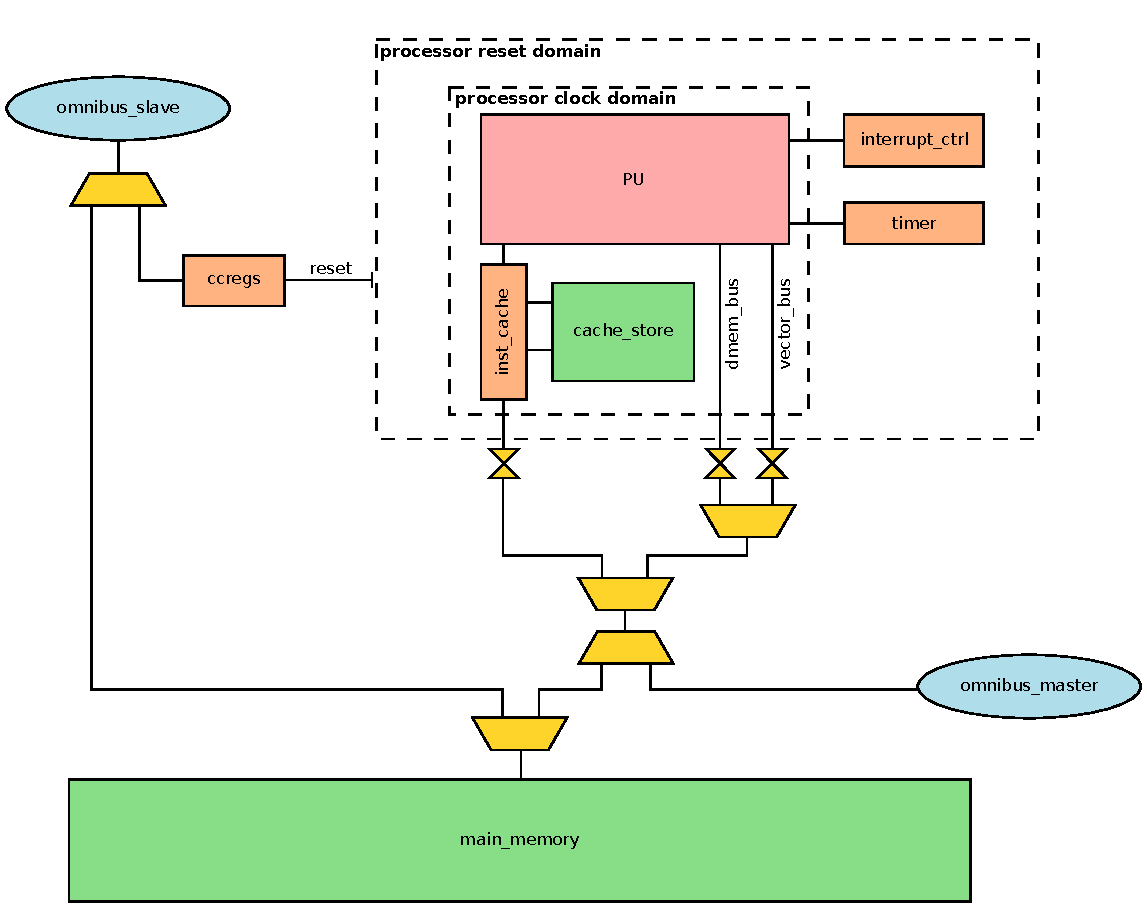
\includegraphics[width=\textwidth]{figures/ppu.pdf}
    \end{center}
    \caption[PPU instantiation example with environment]{%
        Example of environment for Nux as \gls{ppu}.
        The top-level module \code{Pu_v2} is shown as the red block labeled PU.
        The shown configuration uses a shared main memory with instruction cache.
        Data memory, instruction cache, and \gls{fxv} serial load/store all share access to the single main memory block.
        The yellow symbols represent \gls{omnibus} modules.
        A slave port allows access from the outside to change control registers (reset, clock gating) and to main memory (program loading, result retrieval).
        A master port allows access from within the \gls{ppu} to an external bus.
        The \code{interrupt_ctrl} and \code{timer} units implement interrupts and timing.
        They exist outside the clock domain controlled by control registers, but within the reset domain.
    }
    \label{fig:ppuinst}
\end{figure}

Figure~\ref{fig:ppuinst} shows an example of a simple core environment using a shared main memory.

    \chapter{Running software on Nux}
\label{ch:usesw}

Executing a program on Nux in hardware or simulation requires three steps outlined in the next three sections.
First, you have to build a cross-compiler for the PowerISA.
If you want to use \gls{fxv} instructions, binutils needs to be patched.
For the actual execution implementation specific software is required to interface with Nux.


\section{Building a cross-compiler}
Any cross-compiler will do that emits code for the target triple ``powerpc-linux-eabi'', i.e.\ Power instruction set architecture using the \gls{eabi} \citep{IBM1998} for Linux.
Although the latter is probably irrelevant.
In the repository an installation script is provided to compile gcc from source (\file{support/gcc/install.sh}).
You may want to change the \code{PREFIX} variable at the top to select the target installation directory.
You may also want to select newer package versions if available or modify mirror locations if there are errors while downloading.
System libraries (e.g.\ mpfr, gmp, mpc, \ldots) should be used over manually compile ones.
Refer to \cite{installgcc} for required minimum versions.

The goal of the installation script is to build a minimal gcc with support for C but without libc.


\section{Patching binutils for vector operations}

A patch for binutils is provided in directory \file{support/binutils/}.
To apply use patch:
\begin{lstlisting}[language=bash]
    $ tar jxf binutils-2.25.tar.bz2
    $ patch -p0 <binutils-2.25.patch
\end{lstlisting}
Then compile using the install script.

This patch simply adds the non-standard \gls{fxv} instructions to the PowerPC opcode table in binutils.
It thereby enables support for these instructions by the assembler and disassembler (\texttt{objdump -d}).
Therefore, instructions can also be used in gcc inline assembly.


\section{Compiling programs}

The processor starts execution after reset is released at address 0.
Also, exceptions trigger a control transfer to fixed locations in the range from address 4 to 44.
The final result of compilation is therefore to generate a binary image that can be written to memory with valid code at the correct addresses.
This is achieved by a special linker script \code{linker.x} and an assembler wrapper \code{cshell.s}.


\subsection{Assembly wrapper for C code}
An example wrapper is discussed below:
\begin{lstlisting}[language=powerasm]
# chsell.s -- part a
.extern start 
.extern reset
.extern _isr_undefined
.extern isr_einput
.extern isr_alignemnt
.extern isr_program
.extern isr_doorbell
.extern isr_fit
.extern isr_dec

.extern stack_ptr_init
\end{lstlisting}
This declares symbols that can be overwritten by other parts of the program.
The \code{start} symbol declared on line 2 is the entry point for the C code.
It is defined by declaring a function \texttt{void start()} in your C code.
The \code{isr_*} symbols on lines 5 to 10 represent interrupt service routines.
The \code{_isr_undefined} symbol is a default handler that is used if no service routine is defined.

\begin{lstlisting}[language=powerasm]
# chsell.s -- part b
.text
.extern _start:
reset:
	b __init

	# interrupt jump table
	int_mcheck:    b _isr_undefined
	int_cinput:    b _isr_undefined
	int_dstorage:  b _isr_undefined
	int_istorage:  b _isr_undefined
	int_einput:    b isr_einput
	int_alignment: b isr_alignment 
	int_program:   b isr_program
	int_syscall:   b _isr_undefined
	int_doorbell:  b isr_doorbell
	int_cdoorbell: b _isr_undefined
	int_fit:       b isr_fit
	int_dec:       b isr_dec
\end{lstlisting}
This block is the start of the code section of the binary.
It begins on line 5 with a branch to the \code{__init} symbol defined below.
The linker script ensures that this instruction resides at address 0 of the produced binary image.
After that follows the interrupt jump table on lines 8 through 19.
It consists of branches to interrupt service routines, which are located at the appropriate addresses defined by the hardware implementation.


\begin{lstlisting}[language=powerasm]
# chsell.s -- part c
__init:
	# set the stack pointer
	lis 1, stack_ptr_init@h
	addi 1, 1, stack_ptr_init@l
	# start actual program
	bl start

end_loop:
	wait
	b end_loop
\end{lstlisting}
This fragment initialises the stack pointer in general-purpose register 1 as defined by the \gls{eabi} \citep{IBM1998}.
The symbol \code{stack_ptr_init} is defined by the linker script to match the size of the implemented memory.
After initialization on line 7, the wrapper calls the user code at the \code{start} symbol.
If user code returns from the start() function, the loop at the end sends the processor to sleep.
In case of wake-up events, the appropriate service routine will be taken through the interrupt jump table.
On return from the service routine, the branch on line 11 ensures a return to the sleep state.


\subsection{Linker script}
The linker script \code{linker.x} is passed to the linker to configure how the resulting binary is generated.
An example is discussed below:

\begin{lstlisting}
MEMORY {
	ram(rwx) : ORIGIN = 0, LENGTH = 16K
}
\end{lstlisting}
This specifies the memory layout of the implementation.
In the given case we have one memory region with a size of \unit[16]{kib} starting at address 0.
In a tight memory configuration ($ \code{OPT_MEM} = \code{Pu_types::MEM_TIGHT}$) there would be two locations here for data and code.


\begin{lstlisting}
mailbox_size = 4096;
mailbox_end = 0x4000;
mailbox_base = mailbox_end - mailbox_size;
stack_ptr_init = mailbox_base - 8;
\end{lstlisting}
The intention here is to create a reserved memory region at the end called mailbox.
This is used for communication with the environment by software running on Nux.
The stack pointer is initialized to start at lower addresses than the mailbox region.
Note, that the \file{cshell.s} wrapper uses the \code{stack_ptr_init} symbol to do the actual initialization of register 1.


\begin{lstlisting}
SECTIONS {
	.text : {
        _isr_undefined = .;

        *cshell.o(.text)
        *(.text)

        PROVIDE(isr_einput = _isr_undefined);
        PROVIDE(isr_alignment = _isr_undefined);
        PROVIDE(isr_program = _isr_undefined);
        PROVIDE(isr_doorbell = _isr_undefined);
        PROVIDE(isr_fit = _isr_undefined);
        PROVIDE(isr_dec = _isr_undefined);
	} > ram

	.data : {
		*(.data)
		*(.rodata)
	} > ram

	.bss : {
		*(.bss)
		*(.sbss)
	} > ram

  /DISCARD/ : {
    *(.eh_frame)
  }
}
\end{lstlisting}
This part specifies, where generated code sections should be mapped.
We use only the three sections \code{text} for instructions, \code{data} for data, and \code{bss} for zeroed data.
Line 5 ensures, that the wrapper is positioned at memory location 0, so that reset and interrupt handling work correctly.
Line 3 defines the default interrupt handler \code{_isr_undefined} to be equivalent to the reset vector at address 0.
Lines 8 to 13 connect the default handler to all interrupt service routines that were not defined in user code.


\subsection{Minimum user code}

Minimal C user code consists of just the start() function:
\begin{lstlisting}[language=c]
    void start() {
    }
\end{lstlisting}
\subsection{Generating the binary image}

Generating the final binary image involves three steps:
\begin{enumerate}
    \item Compile source files to object files.
    \item Link object files to executable.
    \item Extract binary image of \code{.text} and \code{.data} sections out of the executable.
\end{enumerate}

The following examples assume an architecture with single main memory as shown in Figure~\ref{fig:ppuinst}.
When using two memories, two images have to be extracted at the end, which requires a different \code{linker.x} file as the one shown above.
The examples also assume, that gcc binaries are visible through the \code{PATH} variable and that it was installed with prefix \code{powerpc-linux-eabi}.


\subsubsection{Compiling}

The assembly wrapper has to be assembled:
\begin{lstlisting}
    $ powerpc-linux-eabi-as -mpower7 cshell.s -o cshell.o
\end{lstlisting}
And C-source compiled:
\begin{lstlisting}
    $ powerpc-linux-eabi-gcc -c <sourcefile> -o <objectfile> \
        -ffreestanding   \
        -msdata=none     \
        -mstrict-align   \
        -msoft-float     \
        -mno-relocatable
\end{lstlisting}
The exact meaning of options is given in \cite{gccmanual}.
The first option on line 2 tells the compiler to use a ``freestanding'' environment.
From the gcc manual:
\begin{quote}
   A freestanding environment is one in which the standard library may not exist, and program startup may not necessarily be at main.
   The most obvious example is an OS kernel. 
\end{quote}
Line 3 disables the use of the \code{.sdata} (small data) section in generated code.
Refer to \cite{IBM1998} to learn how this section would be used.
Line 4 avoids unaligned memory accesses.
The PowerISA allows embedded implementations to raise an exception on unaligned loads and stores, which is what this implementation does.
Line 5 disables the use of floating point instructions.
Floating point math is instead implemented in software.
Line 6 tells the compiler, that code may not be relocated to a different address at runtime.


\subsubsection{Linking}

The executable is generated by the linker:
\begin{lstlisting}
    $ powerpc-linux-eabi-ld cshell.o <obj1.o> ... -o <binary.elf> \
        -T linker.x  \
        -static      \
        -nostdlib    \
        -lgcc
\end{lstlisting}
Line 2 tells the linker to use a specified linker script.
Line 3 uses static linking of libraries.
Line 4 disables linking of standard libraries, especially libc (which we do not have).
Line 5 links libgcc.
This is a gcc internal library with routines that the compiler might use instead of directly emitting code for them.
For example, optimized implementations of \code{memcpy} or soft floating point implementations.
See \cite{libgcc} for more information.


\subsubsection{Extracting the binary image}

The objcopy command from binutils allows to extract the raw bits from the executable:
\begin{lstlisting}
    $ powerpc-linux-eabi-objcopy -O binary <binary.elf> <image.raw>
\end{lstlisting}


\subsection{Useful commands}

To inspect the resulting image you can use the hexdump program:
\begin{lstlisting}
    $ hexdump -C <image.raw>
\end{lstlisting}
It outputs a hex-dump to stdout.

The executable can be inspected using readelf to get information about symbol (variables and functions) locations.
Objdump contains a dissasembler:
\begin{lstlisting}
    $ powerpc-linux-eabi-objdump -d <binary.elf>
\end{lstlisting}


\section{Loading and executing programs}

The specifics of how to do this are defined by the system, in which the processor is used.
The binary image generated using objcopy has to be transferred to the memory in the system.
During this time, the processor should be in reset, or you have to know what you are doing.
After loading, reset is released to start the program.
The \code{cshell.s} wrapper ensures, that the program goes into the sleep state when the user code terminates, i.e.\ returns from the start() function.





    % Outline
    %\chapter{Design Implementation Overview}
    %\section{Frontend}
    %\section{Functional units}
    %\section{Peripheral logic}

    \chapter{Running simulations}

Available tests are described in detail in Chapter~4 of \cite{friedmann13phd}.
Here, we will focus on how to use theses tests.
In order to do that, we will also discuss the Makefile-based build flow.


\section{Build flow}
The build flow uses \code{make} and was inspired by the Linux build system kbuild \citep{kbuild}.
There is a central configuration file \file{.config} in the top-level directory that defines configuration options.
Source files are collected by using \file{Makefile.srclist} files throughout the directory hierarchy using the configured options.
Separate files \code{Makefile.build} hold the build rules for \code{make} for each supported simulator.
These Makefiles reside in run directories under \file{verification/sim_*}.
Currently only ModelSim is supported in \file{verification/sim_model/}.
Run directories for synthesis are located in \file{target/}.


\subsection{Configuration options}

These configuration options can be given in the global configuration file \file{.config}.

\begin{description}
    \item[\code{CONFIG_PLATFORM}] \textit{= [~virtex5 | tsmc65 | umc180 | designware | achronix\_speedster22ihd~]}

        Select the target technology.
        Some components for clock generation, memories, multipliers, etc.\ only work in particular technologies, for example when using specialized \gls{fpga} resources.
        Note, that support for the achronix \gls{fpga} is merely a placeholder.

    \item[\code{CONFIG_BOARD}] \textit{= [~ml505 | flyspi-board~]}

        Select which \gls{fpga} board is used.
        The Xilinx evaluation board ml505 \citep{ml505_ug_2008} or the ``flyspi'' board of the electronic vision(s) group.
        Support for the latter is preliminary.
        This option is only relevant for the \file{target/emsys} implementation run directory.

    \item[\code{CONFIG_USE_XILINX_MULTIPLIER}] \textit{= [~y | n~]}

        Select whether to use integrated DSP slices, when building for \code{CONFIG_PLATFORM} = virtex5.

    \item[\code{CONFIG_WITH_BUS}] \textit{= [~y | n~]}

        Build the \gls{omnibus} implementation provided as part of the repository or not.


    \item[\code{CONFIG_WITH_VECTOR}] \textit{= [~y | n~]}

        Build modules for the \gls{fxv} unit or not.
\end{description}


\subsection{Running simulations}

To compile sources for simulation with ModelSim according to the selected configuration do:
\begin{lstlisting}[language=bash]
   $ cd verification/sim_model
   $ make
   $ vsim -do <simulation script>
\end{lstlisting}
Several simulation scripts are provided for the different test scenarios.

\section{Tests}

\subsection{Program test}

\begin{tabular}{ll}
    \textit{Simulation script:}     & \file{verification/sim_model/sim_plt.do} \\
    \textit{Top-level source:}      & \file{testbenches/program_test.sv} \\
\end{tabular} \\
This test executes a number of programs from \file{test/testcode}.
The processor is simulated in a two memory environment.
Therefore, each program provides code and memory images, plus an additional expected data image.
The test compares the memory contents after simulation to the expected image.
Memory images can be provided as ASCII files with hexadecimal values or in raw binary form.
For new programs the latter format should be preferred, since it can be generated using the flow described in Chapter~\ref{ch:usesw}.


\subsection{Sequence test}

\begin{tabular}{ll}
    \textit{Simulation script:}     & \file{verification/sim_model/sim_seq.do} \\
    \textit{Top-level source:}      & \file{testbenches/sequence_test.sv} \\
\end{tabular} \\
This test generates random program sequences and compares the final state of internal registers to the expected state.
\Gls{fxv} instructions are excluded from random generation.
Also the \code{tw} and \code{twi} instructions are not allowed to avoid exceptions.
The test can be configured with four preprocessor options:
\begin{description}
    \item[\code{PROGRAM_LENGTH}]
        Number of instructions of which the last one is always \code{wait}.

    \item[\code{OPT_BCACHE}]
        Passed to the top-level processor option of the same name (see Section~\ref{sec:topopt}).

    \item[\code{USE_CACHE}]
        Perform the test using an instruction cache.

    \item[\code{OPT_DMEM_BUS}]
        If set, use $\code{OPT_DMEM} = \code{Pu_types::DMEM_BUS}$ (see Section~\ref{sec:topopt}).
\end{description}
The simulation itself runs indefinitely.
Specify a time when starting the simulation.
For good coverage a simulated time of \unit[100]{ms} should be aimed for.


\subsection{Vector unit test}
\begin{tabular}{ll}
    \textit{Simulation script:}     & \file{verification/sim_model/sim_fub_vector.do} \\
    \textit{Top-level source:}      & \file{testbenches/fub_vector_test.sv} \\
\end{tabular} \\
This is a unit test for the vector unit.
It tests the design in three phases:
\begin{enumerate}
    \item Explicitly specified programs.
    \item Randomly generated single instructions.
    \item Randomly generated sequences of instructions.
\end{enumerate}
A larger test set is defined by \file{testbenches/signoff_vector_test.sv} that includes the top-level of this test.
The simulation script \file{verification/sim_model/sim_signoff_vector_test.do} uses this as top-level.

    \chapter{Instruction set}

\minitoc

\section{Implemented subset of Power ISA 2.06}

\cite{powerisa_206} defines an embedded and a server environment, several mandatory and optional categories for these environments, and allows \unit[32 and 64]{bit} implementations.
The presented processor realizes an embedded environment supporting categories Base, Embedded, External Control, and Wait using \unit[32]{bit}.
In addition it supports the custom \gls{fxv} instruction set and two now deprecated instruction sets \gls{never} and \gls{synapse}.
The full list of implemented instructions is given in \cite{friedmann13phd}.

Opcodes and instruction formats are defined in source file \file{rtl/packages/pu_inst_pkg.sv}.
The high-level behavior, e.g.\ what registers are read and written or which functional unit is used, is given by the predecode module in \file{rtl/processor/predecode.sv}.


\section{FXV vector instruction set}

This section lists the implemented instructions of the fixed-point vector functional unit of Nux.
The following rules are used in the notation:
\begin{itemize}
    \item Round brackets indicate the contents of the register selected by the index in brackets.
        So, $(\text{VRA})$ stands for the contents of the register with index VRA.
    \item Subscripts denote the element of the vector using the current type:
        $(\text{VRA})_{i/8}$ is the $i-\text{th}$ halfword element, $(\text{VRA})_{i/16}$ is the $i-\text{th}$ byte element, and $(\text{VRA})_{i/32}$ is the $i-\text{th}$ half-byte element.
    \item Lowercase letters $u, v, w, m$ indicate single-precision elements.
        Uppercase letters $U, V, W, M$ are double-precision elements.
    \item Underlined letters $\underline{u}, \underline{v}$ indicate full single-precision vectors.
    \item VRA, VRB, and VRT refer to vector register indices.
    \item ACC is the contents of the double-precision accumulation register.
    \item VCR is contents of the \unit[32]{bit} vector condition register.
    \item RA, RB refer to general-purpose registers.
\end{itemize}

\subsection{Registers}

\subsubsection{Vector register file (VRF)}

\begin{bytefield}[bitwidth=0.2em]{128}
    \bitheader{0,31,63,95,127} \\
    \bitbox{16}{$\text{VR0}_{0/8}$} & \bitbox{16}{$\text{VR0}_{1/8}$}  & \bitbox{16}{$\text{VR0}_{2/8}$} & \bitbox{16}{$\text{VR0}_{3/8}$} & \bitbox{16}{$\text{VR0}_{4/8}$} & \bitbox{16}{$\text{VR0}_{5/8}$} & \bitbox{16}{$\text{VR0}_{6/8}$} & \bitbox{16}{$\text{VR0}_{7/8}$}\\
    \bitbox{128}{$\vdots$} \\
    \bitbox{128}{VR31} \\
\end{bytefield} \\
The vector register file contains 32 \unit[128]{bit} vector registers, which consist of 8 halfword elements.
Each element can also be used as two byte elements depending on the used instruction.


\subsubsection{Vector condition register (VCR)}

\begin{bytefield}[bitwidth=0.2em]{96}
    \bitheader{0,11,23,35,47,59,71,83,95} \\
    \bitbox{12}{$C_0$}   %
    & \bitbox{12}{$C_1$} %
    & \bitbox{12}{$C_2$} %
    & \bitbox{12}{$C_3$} %
    & \bitbox{12}{$C_4$} %
    & \bitbox{12}{$C_5$} %
    & \bitbox{12}{$C_6$} %
    & \bitbox{12}{$C_7$} \\
\end{bytefield} \\
The vector condition register has one field for each of the 8 halfword elements:

\begin{bytefield}[bitwidth=1em]{12}
    \bitheader{0,3,4,7,8,11} \\
    \bitbox{4}{EQ} & \bitbox{4}{GT} & \bitbox{4}{LT} \\
    {\footnotesize %
    \bitbox{1}{0}   %
    & \bitbox{1}{1} %
    & \bitbox{1}{2} %
    & \bitbox{1}{3} %
    & \bitbox{1}{0} %
    & \bitbox{1}{1} %
    & \bitbox{1}{2} %
    & \bitbox{1}{3} %
    & \bitbox{1}{0} %
    & \bitbox{1}{1} %
    & \bitbox{1}{2} %
    & \bitbox{1}{3} } \\
\end{bytefield} \\
Each field consists of three condition areas for equality (EQ), greater than (GT), and less than (LT).
For each nibble (\unit[4]{bit}) in the vector one condition bit is stored.
Note: nibble-wise condition bits are a leftover from early days.
Currently, there is no way to set or use them individually.
Operations use two or four bits simultaneously for byte or halfword operations.


\subsection{Primitive functions}
Some instructions take only effect for individual elements if a given condition is met.
The condition is determined by the contents of the vector condition register and the condition field in the instruction in the following way:
{\footnotesize
\begin{algorithmic}[1]
    \Function {conditional}{cond, vcr\_field}
        \If { cond = 0 }
            \State \Return true
        \ElsIf { cond = 1 }
            \State \Return vcr\_field.gt
        \ElsIf { cond = 2 }
            \State \Return vcr\_field.lt
        \ElsIf { cond = 3 }
            \State \Return vcr\_field.eq
        \EndIf
    \EndFunction
\end{algorithmic} }


\paragraph{Shift and logical functions}
The $\text{\sc{shift\_left}}(x,n)$ function gives the result of shifting $x$ left by $n$ positions while filling in zeros on the right.
Shifted-out bits are discarded.

The $\text{\sc{shift\_right}}(x,n)$ function gives the result of shifting $x$ right by $n$ positions while filling in zeros on the left.

The $\text{\sc{sign\_extend}}(x)$ function gives the result of sign extending $x$ to the width of the assignee of this function.

The $\text{\sc{bitwise\_and}}(a, b)$ function represents the result of performing a bitwise and between $a$ and $b$.

The $\text{\sc{bitwise\_or}}(a, b)$ function represents the result of performing a bitwise or between $a$ and $b$.

\paragraph{Saturating and fractional arithmetic}
Some instructions use fractional representation usually combined with saturating arithmetics.
The function below defines saturating multiplication of two fractional operands of \unit[$n$]{bit} size.
The result is \unit[$2n$]{bit} wide and shifted to the left to get rid of one superfluous sign bit.
Saturation only occurs if both operands represent $-1$ ($= 100\ldots 0$ in binary).
{\footnotesize
\begin{algorithmic}[1]
    \Function {mult\_sat\_fract}{a, b, n}
        \If { $a = -2^{n-1} \land b = -2^{n-1}$ }
            \State \Return $2^{2*n-1} - 1$
        \Else
            \State $u \gets a \cdot b$
            \State \Return \Call{shift\_left}{$u$, 1}
        \EndIf
    \EndFunction
\end{algorithmic} }

The following function defines saturating addition of two \unit[$n$]{bit} operands.
In case of overflows, the result saturates to the maximum and minimum representable value.
{\footnotesize
\begin{algorithmic}[1]
    \Function {add\_sat}{a, b, n}
        \State $y \gets a + b$
        \If { $y > 2^{n-1} - 1$ }
            \State \Return $2^{n-1} - 1$
        \ElsIf { $y < -2^{n-1}$ }
            \State \Return $-2^{n-1}$
        \Else
            \State \Return $y$
        \EndIf
    \EndFunction
\end{algorithmic} }


\paragraph{Memories and IO}
Function $\text{\sc{mem}}(a)$ represents the \unit[32]{bit }contents of main memory at address $a$.

Function $\text{\sc{io}}(a)$ represents the contents of \gls{io} location $a$.
The width of this result is determined by the width of vectors (\code{OPT_VECTOR_NUM_HALFWORDS}) and the number of slices (\code{OPT_VECTOR_SLICES}).


\begin{multicols}{2}[%
    \subsection{Modulo halfword instructions}%
]

\fxvinst{Multiply accumulate halfword modulo}{fxvmahm}{12}{%
    \For {$0 \le i < 8$}
        \State $u \gets (\text{VRA})_{i/8}$
        \State $v \gets (\text{VRB})_{i/8}$
        \State $W \gets u \cdot v$
        \State $M \gets \text{ACC}_{i/8}$
        
        \State enable $\gets$ \Call{conditional}{C, VCR$_{i/8}$}

        \If { enable }
            \State $(\text{VRT})_{i/8} \gets W + M_i \mod 2^{16}$
        \EndIf

    \EndFor
}{%
    The contents of vector registers VRA and VRB are multiplied as \unit[16]{bit} halfword elements and added to the contents of the \unit[32]{bit} double-precision accumulation register.
    The result is written to vector register VRT modulo $2^{16}$ if the specified condition is met.
}

\fxvinst{Multiply accumulate to accumulator halfword modulo}{fxvmatachm}{44}{%
    \For {$0 \le i < 8$}
        \State $u \gets (\text{VRA})_{i/8}$
        \State $v \gets (\text{VRB})_{i/8}$
        \State $W \gets u \cdot v$
        \State $M \gets \text{ACC}_{i/8}$

        \State enable $\gets$ \Call{conditional}{C, VCR$_{i/8}$}

        \If { enable }
            \State $\text{ACC}_{i/8} \gets W + M_i \mod 2^{32}$
        \EndIf

    \EndFor
}{%
    The contents of vector registers VRA and VRB are multiplied as \unit[16]{bit} halfword elements and added to the contents of the \unit[32]{bit} double-precision accumulation register.
    The result is written to the accumulation register modulo $2^{32}$ if the specified condition is met.
}

\fxvinst{Multiply halfword modulo}{fxvmulhm}{76}{%
    \For {$0 \le i < 8$}
        \State $u \gets (\text{VRA})_{i/8}$
        \State $v \gets (\text{VRB})_{i/8}$

        \State enable $\gets$ \Call{conditional}{C, VCR$_{i/8}$}

        \If { enable }
            \State $(\text{VRT})_{i/8} \gets u \cdot v \mod 2^{16}$
        \EndIf
    \EndFor
}{%
    The contents of vector registers VRA and VRB are multiplied as \unit[16]{bit} halfword elements.
    The result is written to the vector register indicated by VRT modulo $2^{16}$ if the specified condition is met.
}

\fxvinst{Multiply to accumulator halfword modulo}{fxvmultachm}{108}{%
    \For {$0 \le i < 8$}
        \State $u \gets (\text{VRA})_{i/8}$
        \State $v \gets (\text{VRB})_{i/8}$

        \State enable $\gets$ \Call{conditional}{C, VCR$_{i/8}$}

        \If { enable }
            \State $\text{ACC}_{i/8} \gets u \cdot v \mod 2^{32}$
        \EndIf
    \EndFor
}{%
    The contents of vector registers VRA and VRB are multiplied as \unit[16]{bit} halfword elements.
    The result is written to the accumulator modulo $2^{32}$ if the specified condition is met.
}

\fxvinst{Subtract halfword modulo}{fxvsubhm}{332}{%
    \For {$0 \le i < 8$}
        \State $u \gets (\text{VRA})_{i/8}$
        \State $v \gets (\text{VRB})_{i/8}$

        \State enable $\gets$ \Call{conditional}{C, VCR$_{i/8}$}

        \If { enable }
            \State $(\text{VRT})_{i/8} \gets u - v \mod 2^{16}$
        \EndIf
    \EndFor
}{%
    The contents of the vector register indicated by VRB is subtracted from the contents of the register indicated by VRA.
    The result is written to VRT modulo $2^{16}$ if the specified condition is met.
}

\fxvinst{Add accumulator to accumulator halfword modulo}{fxvaddactachm}{364}{%
    \For {$0 \le i < 8$}
        \State $U \gets \Call{sign\_extend}{(\text{VRA})_{i/8}}$
        \State $M \gets ACC_{i/8}$

        \State enable $\gets$ \Call{conditional}{C, VCR$_{i/8}$}

        \If { enable }
            \State $\text{ACC}_{i/8} \gets U + M \mod 2^{32}$
        \EndIf
    \EndFor
}{%
    The contents of vector register VRA is sign extended to double precision and added to the accumulation register.
    The result is written to the accumulator modulor $2^{32}$ if the specified condition is met.
}

\fxvinst{Add and save to accumulator halfword modulo}{fxvaddtachm}{428}{%
    \For {$0 \le i < 8$}
        \State $U \gets \Call{sign\_extend}{(\text{VRA})_{i/8}}$
        \State $V \gets \Call{sign\_extend}{(\text{VRB})_{i/8}}$

        \State enable $\gets$ \Call{conditional}{C, VCR$_{i/8}$}

        \If { enable }
            \State $\text{ACC}_{i/8} \gets U + V$
        \EndIf
    \EndFor
}{%
    The contents of vector registers VRA and VRB are sign extended to double precision.
    If the specified condition is met, their sum is written to the accumulator.
}

\fxvinst{Add accumulator halfword modulo}{fxvaddachm}{396}{%
    \For {$0 \le i < 8$}
        \State $U \gets \Call{sign\_extend}{(\text{VRA})_{i/8}}$
        \State $M \gets \text{ACC}_{i/8}$

        \State enable $\gets$ \Call{conditional}{C, VCR$_{i/8}$}

        \If { enable }
            \State $(\text{VRT})_{i/8} \gets U + M \mod 2^{16}$
        \EndIf
    \EndFor
}{%
    The contents of vector register VRA is sign extended to double precision and added to the accumulator.
    The result is written to vector register VRT modulo $2^{16}$.
}

\fxvinst{Add halfword modulo}{fxvaddhm}{460}{%
    \For {$0 \le i < 8$}
        \State $U \gets \Call{sign\_extend}{(\text{VRA})_{i/8}}$
        \State $V \gets \Call{sign\_extend}{(\text{VRB})_{i/8}}$

        \State enable $\gets$ \Call{conditional}{C, VCR$_{i/8}$}

        \If { enable }
            \State $(\text{VRT})_{i/8} \gets U + V \mod 2^{16}$
        \EndIf
    \EndFor
}{%
    The contents of vector registers indicated by VRA and VRB are added.
    If the specified condition is met, the result is written to the vector register indicated by VRT.
}

\fxvinst{Compare halfword modulo}{fxvcmphm}{300}{%
    \For {$0 \le i < 8$}
        \State $u \gets (\text{VRA})_{i/8}$
        \State $\text{VCR}_{i/8}.eq \gets u = 0$
        \State $\text{VCR}_{i/8}.gt \gets u > 0$
        \State $\text{VCR}_{i/8}.lt \gets u < 0$
    \EndFor
}{%
    The contents of the vector register indicated by VRA is compared to zero and the result written to the vector condition register.
}


\fxvinst{Move to accumulator halfword fractional}{fxvmtach}{15}{%
    \For {$0 \le i < 8$}
        \State enable $\gets$ \Call{conditional}{C, VCR$_{i/8}$}

        \If { enable }
            \State $(\text{ACC})_{i/8} \gets (\text{VRA})_{i/8}$
        \EndIf
    \EndFor
}{%
    If enabled, the contents of elements in register VRA are copied to the accumulator aligned to the right.
}


\fxvinstGPRa{Splat halfword}{fxvsplath}{268}{%
    \For {$0 \le i < 8$}
        \State $u \gets \text{RA} \mod 2^{16}$
        \State $\text{VRT}_{i/8} \gets u$
    \EndFor
}{%
    The lower halfword of general-purpose register RA is copied to each element of VRT.
}
\end{multicols}

\begin{multicols}{2}[%
    \subsection{Modulo byte instructions}%
]

\fxvinst{Multiply accumulate byte modulo}{fxvmabm}{13}{%
    \For {$0 \le i < 16$}
        \State $u \gets (\text{VRA})_{i/16}$
        \State $v \gets (\text{VRB})_{i/16}$
        \State $W \gets u \cdot v$
        \State $M \gets \text{ACC}_{i/16}$
        
        \State enable $\gets$ \Call{conditional}{C, VCR$_{i/16}$}

        \If { enable }
            \State $(\text{VRT})_{i/16} \gets W + M_i \mod 2^{8}$
        \EndIf

    \EndFor
}{%
    The contents of vector registers VRA and VRB are multiplied as \unit[8]{bit} byte elements and added to the contents of the \unit[16]{bit} double-precision accumulation register.
    The result is written to vector register VRT modulo $2^{8}$ if the specified condition is met.
}

\fxvinst{Multiply accumulate to accumulator byte modulo}{fxvmatacbm}{45}{%
    \For {$0 \le i < 16$}
        \State $u \gets (\text{VRA})_{i/16}$
        \State $v \gets (\text{VRB})_{i/16}$
        \State $W \gets u \cdot v$
        \State $M \gets \text{ACC}_{i/16}$

        \State enable $\gets$ \Call{conditional}{C, VCR$_{i/16}$}

        \If { enable }
            \State $\text{ACC}_{i/16} \gets W + M_i \mod 2^{16}$
        \EndIf

    \EndFor
}{%
    The contents of vector registers VRA and VRB are multiplied as \unit[8]{bit} byte elements and added to the contents of the \unit[16]{bit} double-precision accumulation register.
    The result is written to the accumulation register modulo $2^{16}$ if the specified condition is met.
}

\fxvinst{Multiply byte modulo}{fxvmulbm}{77}{%
    \For {$0 \le i < 16$}
        \State $u \gets (\text{VRA})_{i/16}$
        \State $v \gets (\text{VRB})_{i/16}$

        \State enable $\gets$ \Call{conditional}{C, VCR$_{i/16}$}

        \If { enable }
            \State $(\text{VRT})_{i/16} \gets u \cdot v \mod 2^{8}$
        \EndIf
    \EndFor
}{%
    The contents of vector registers VRA and VRB are multiplied as \unit[8]{bit} byte elements.
    The result is written to the vector register indicated by VRT modulo $2^{8}$ if the specified condition is met.
}

\fxvinst{Multiply to accumulator byte modulo}{fxvmultacbm}{109}{%
    \For {$0 \le i < 16$}
        \State $u \gets (\text{VRA})_{i/16}$
        \State $v \gets (\text{VRB})_{i/16}$

        \State enable $\gets$ \Call{conditional}{C, VCR$_{i/16}$}

        \If { enable }
            \State $\text{ACC}_{i/16} \gets u \cdot v \mod 2^{16}$
        \EndIf
    \EndFor
}{%
    The contents of vector registers VRA and VRB are multiplied as \unit[8]{bit} byte elements.
    The result is written to the accumulator modulo $2^{16}$ if the specified condition is met.
}

\fxvinst{Subtract byte modulo}{fxvsubbm}{333}{%
    \For {$0 \le i < 16$}
        \State $u \gets (\text{VRA})_{i/16}$
        \State $v \gets (\text{VRB})_{i/16}$

        \State enable $\gets$ \Call{conditional}{C, VCR$_{i/16}$}

        \If { enable }
            \State $(\text{VRT})_{i/16} \gets u - v \mod 2^{8}$
        \EndIf
    \EndFor
}{%
    The contents of the vector register indicated by VRB is subtracted from the contents of the register indicated by VRA.
    The result is written to VRT modulo $2^{8}$ if the specified condition is met.
}

\fxvinst{Add accumulator to accumulator byte}{fxvaddactacb}{365}{%
    \For {$0 \le i < 16$}
        \State $U \gets \Call{sign\_extend}{(\text{VRA})_{i/16}}$
        \State $M \gets ACC_{i/16}$

        \State enable $\gets$ \Call{conditional}{C, VCR$_{i/16}$}

        \If { enable }
            \State $\text{ACC}_{i/16} \gets U + M \mod 2^{16}$
        \EndIf
    \EndFor
}{%
    The contents of vector register VRA is sign extended to double precision and added to the accumulation register.
    The result is written to the accumulator modulo $2^{16}$ if the specified condition is met.
}

\fxvinst{Add and save to accumulator byte modulo}{fxvaddtacb}{429}{%
    \For {$0 \le i < 16$}
        \State $U \gets \Call{sign\_extend}{(\text{VRA})_{i/16}}$
        \State $V \gets \Call{sign\_extend}{(\text{VRB})_{i/16}}$

        \State enable $\gets$ \Call{conditional}{C, VCR$_{i/16}$}

        \If { enable }
            \State $\text{ACC}_{i/16} \gets U + V$
        \EndIf
    \EndFor
}{%
    The contents of vector registers VRA and VRB are sign extended to double precision.
    If the specified condition is met, their sum is written to the accumulator.
}

\fxvinst{Add accumulator byte modulo}{fxvaddacbm}{397}{%
    \For {$0 \le i < 16$}
        \State $U \gets \Call{sign\_extend}{(\text{VRA})_{i/16}}$
        \State $M \gets \text{ACC}_{i/16}$

        \State enable $\gets$ \Call{conditional}{C, VCR$_{i/16}$}

        \If { enable }
            \State $(\text{VRT})_{i/16} \gets U + M \mod 2^{8}$
        \EndIf
    \EndFor
}{%
    The contents of vector register VRA is sign extended to double precision and added to the accumulator.
    The result is written to vector register VRT modulo $2^{8}$.
}

\fxvinst{Add byte modulo}{fxvaddbm}{461}{%
    \For {$0 \le i < 16$}
        \State $U \gets \Call{sign\_extend}{(\text{VRA})_{i/16}}$
        \State $V \gets \Call{sign\_extend}{(\text{VRB})_{i/16}}$

        \State enable $\gets$ \Call{conditional}{C, VCR$_{i/16}$}

        \If { enable }
            \State $(\text{VRT})_{i/16} \gets U + V \mod 2^{8}$
        \EndIf
    \EndFor
}{%
    The contents of vector registers indicated by VRA and VRB are added.
    If the specified condition is met, the result is written to the vector register indicated by VRT.
}

\fxvinst{Compare byte}{fxvcmpb}{301}{%
    \For {$0 \le i < 16$}
        \State $u \gets (\text{VRA})_{i/16}$
        \State $\text{VCR}_{i/16}.eq \gets u = 0$
        \State $\text{VCR}_{i/16}.gt \gets u > 0$
        \State $\text{VCR}_{i/16}.lt \gets u < 0$
    \EndFor
}{%
    The contents of the vector register indicated by VRA is compared to zero and the result written to the vector condition register.
}


\fxvinst{Move to accumulator byte}{fxvmtacb}{14}{%
    \For {$0 \le i < 16$}
        \State enable $\gets$ \Call{conditional}{C, VCR$_{i/16}$}

        \If { enable }
            \State $(\text{ACC})_{i/16} \gets (\text{VRA})_{i/16}$
        \EndIf
    \EndFor
}{%
    If enabled, the contents of elements in register VRA are copied to the accumulator aligned to the right.
}


\fxvinstGPRa{Splat byte}{fxvsplatb}{269}{%
    \For {$0 \le i < 16$}
        \State $u \gets \text{RA} \mod 2^{8}$
        \State $\text{VRT}_{i/16} \gets u$
    \EndFor
}{%
    The lower byte of general-purpose register RA is copied to each element of VRT.
}
\end{multicols}

\begin{multicols}{2}[%
    \subsection{Saturating, fractional, halfword instructions}%
]

\fxvinst{Multiply accumulate halfword fractional saturating}{fxvmahfs}{28}{%
    \For {$0 \le i < 8$}
        \State $u \gets (\text{VRA})_{i/8}$
        \State $v \gets (\text{VRB})_{i/8}$
        \State $W \gets \Call{mult\_sat\_fract}{u, v, \unit[16]{bit}}$
        \State $M \gets \Call{add\_sat}{\text{ACC}_{i/8}, W, \unit[32]{bit}}$
        
        \State enable $\gets$ \Call{conditional}{C, VCR$_{i/8}$}

        \If { enable }
            \State $(\text{VRT})_{i/8} \gets \Call{shift\_right}{M, 16}$
        \EndIf

    \EndFor
}{%
    Perform multiplication of registers VRA and VRB using fractional representation and saturating on overflows.
    The double width result is added with the contents of the accumulation register again with saturation on overflow.
    The upper 16 bits of the result are returned to register VRT if the condition is met.
    The accumulation register is not modified.
}


\fxvinst{Move to accumulator halfword fractional}{fxvmtachf}{31}{%
    \For {$0 \le i < 8$}
        \State enable $\gets$ \Call{conditional}{C, VCR$_{i/8}$}

        \If { enable }
            \State $(\text{ACC})_{i/8} \gets (\text{VRA})_{i/8} \cdot 2^{16}$
        \EndIf
    \EndFor
}{%
    If enabled, the contents of elements in register VRA are copied to the accumulator aligned to the left.
}


\fxvinst{Multiply accumulate and save to accumulator halfword fractional}{fxvmatachfs}{60}{%
    \For {$0 \le i < 8$}
        \State $u \gets (\text{VRA})_{i/8}$
        \State $v \gets (\text{VRB})_{i/8}$
        \State $W \gets \Call{mult\_sat\_fract}{u, v, \unit[16]{bit}}$
        \State $M \gets \Call{add\_sat}{\text{ACC}_{i/8}, W, \unit[32]{bit}}$
        
        \State enable $\gets$ \Call{conditional}{C, VCR$_{i/8}$}

        \If { enable }
            \State $(\text{ACC})_{i/8} \gets M$
        \EndIf
    \EndFor
}{%
    Perform a multiply-add operation of registers VRA, VRB, and the accumulator using saturation and fractional arithmetics.
    If enabled, the result is stored in the accumulator.
}


\fxvinst{Multiply halfword fractional saturating}{fxvmulhfs}{92}{%
    \For {$0 \le i < 8$}
        \State $u \gets (\text{VRA})_{i/8}$
        \State $v \gets (\text{VRB})_{i/8}$
        \State $W \gets \Call{mult\_sat\_fract}{u, v, \unit[16]{bit}}$
        
        \State enable $\gets$ \Call{conditional}{C, VCR$_{i/8}$}

        \If { enable }
            \State $(\text{VRT})_{i/8} \gets \Call{shift\_right}{M, 16}$
        \EndIf
    \EndFor
}{%
    Perform saturating multiplication in fractional representation of the contents of registers VRA and VRB.
    Store the truncated result to register VRT if enabled.
}


\fxvinst{Multiply and save to accumulator halfword fractional saturating}{fxvmultachfs}{124}{%
    \For {$0 \le i < 8$}
        \State $u \gets (\text{VRA})_{i/8}$
        \State $v \gets (\text{VRB})_{i/8}$
        \State $W \gets \Call{mult\_sat\_fract}{u, v, \unit[16]{bit}}$
        
        \State enable $\gets$ \Call{conditional}{C, VCR$_{i/8}$}

        \If { enable }
            \State $(\text{ACC})_{i/8} \gets M$
        \EndIf
    \EndFor
}{%
    Perform saturating multiplication in fractional representation of the contents of registers VRA and VRB.
    Store the result to the accumulator.
}


\fxvinst{Subtract halfword fractional saturating}{fxvsubhfs}{348}{%
    \For {$0 \le i < 8$}
        \State $U \gets \Call{sign\_extend}{(\text{VRA})_{i/8}}$
        \State $V \gets \Call{sign\_extend}{- (\text{VRB})_{i/8}}$
        \State $W \gets \Call{add\_sat\_fract}{U, V, \unit[32]{bit}}$
        
        \State enable $\gets$ \Call{conditional}{C, VCR$_{i/8}$}

        \If { enable }
            \State $(\text{VRT})_{i/8} \gets \Call{shift\_right}{W, 16}$
        \EndIf
    \EndFor
}{%
    Add the contents of register VRA to the negated contents of register VRB using saturation.
    Store the truncated result to register VRT if enabled.
}


\fxvinst{Add accumulator and save to accumulator halfword fractional}{fxvaddactachf}{380}{%
    \For {$0 \le i < 8$}
        \State $U \gets \Call{sign\_extend}{(\text{VRA})_{i/8}}$
        \State $V \gets (\text{ACC})_{i/8}$
        \State $W \gets \Call{add\_sat\_fract}{U, V, \unit[32]{bit}}$
        
        \State enable $\gets$ \Call{conditional}{C, VCR$_{i/8}$}

        \If { enable }
            \State $(\text{ACC})_{i/8} \gets W$
        \EndIf
    \EndFor
}{%
    Add the sign extended contents of register VRA to the accumulator using saturating arithmetics and store the result to the accumulator.
}


\fxvinst{Add accumulator halfword fractional saturating}{fxvaddachfs}{412}{%
    \For {$0 \le i < 8$}
        \State $U \gets \Call{sign\_extend}{(\text{VRA})_{i/8}}$
        \State $V \gets (\text{ACC})_{i/8}$
        \State $W \gets \Call{add\_sat\_fract}{U, V, \unit[32]{bit}}$
        
        \State enable $\gets$ \Call{conditional}{C, VCR$_{i/8}$}

        \If { enable }
            \State $(\text{VRT})_{i/8} \gets \Call{shift\_right}{W, 16}$
        \EndIf
    \EndFor
}{%
    Add the sign extended contents of register VRA to the accumulator using saturating arithmetics.
    Store the truncated result to register VRT.
}


\fxvinst{Add halfword fractional saturating}{fxvaddhfs}{476}{%
    \For {$0 \le i < 8$}
        \State $U \gets \Call{sign\_extend}{(\text{VRA})_{i/8}}$
        \State $V \gets \Call{sign\_extend}{(\text{VRB})_{i/8}}$
        \State $W \gets \Call{add\_sat\_fract}{U, V, \unit[32]{bit}}$
        
        \State enable $\gets$ \Call{conditional}{C, VCR$_{i/8}$}

        \If { enable }
            \State $(\text{VRT})_{i/8} \gets \Call{shift\_right}{W, 16}$
        \EndIf
    \EndFor
}{%
    Add the contents of registers VRA and VRB using saturating arithmetics.
    Store the result to register VRT.
}


\end{multicols}


\begin{multicols}{2}[%
    \subsection{Saturating, fractional, byte instructions}%
]

\fxvinst{Multiply accumulate byte fractional saturating}{fxvmabfs}{29}{%
    \For {$0 \le i < 16$}
        \State $u \gets (\text{VRA})_{i/16}$
        \State $v \gets (\text{VRB})_{i/16}$
        \State $W \gets \Call{mult\_sat\_fract}{u, v, \unit[8]{bit}}$
        \State $M \gets \Call{add\_sat}{\text{ACC}_{i/16}, W, \unit[16]{bit}}$
        
        \State enable $\gets$ \Call{conditional}{C, VCR$_{i/16}$}

        \If { enable }
            \State $(\text{VRT})_{i/16} \gets \Call{shift\_right}{M, 8}$
        \EndIf

    \EndFor
}{%
    Perform multiplication of registers VRA and VRB using fractional representation and saturating on overflows.
    The double width result is added with the contents of the accumulation register again with saturation on overflow.
    The upper 8 bits of the result are returned to register VRT if the condition is met.
    The accumulation register is not modified.
}


\fxvinst{Move to accumulator byte fractional}{fxvmtacbf}{30}{%
    \For {$0 \le i < 16$}
        \State enable $\gets$ \Call{conditional}{C, VCR$_{i/16}$}

        \If { enable }
            \State $(\text{ACC})_{i/16} \gets (\text{VRA})_{i/16} \cdot 2^{8}$
        \EndIf
    \EndFor
}{%
    If enabled, the contents of elements in register VRA are copied to the accumulator aligned to the left.
}


\fxvinst{Multiply accumulate and save to accumulator byte fractional}{fxvmatacbfs}{61}{%
    \For {$0 \le i < 16$}
        \State $u \gets (\text{VRA})_{i/16}$
        \State $v \gets (\text{VRB})_{i/16}$
        \State $W \gets \Call{mult\_sat\_fract}{u, v, \unit[8]{bit}}$
        \State $M \gets \Call{add\_sat}{\text{ACC}_{i/16}, W, \unit[16]{bit}}$
        
        \State enable $\gets$ \Call{conditional}{C, VCR$_{i/16}$}

        \If { enable }
            \State $(\text{ACC})_{i/16} \gets M$
        \EndIf
    \EndFor
}{%
    Perform a multiply-add operation of registers VRA, VRB, and the accumulator using saturation and fractional arithmetics.
    If enabled, the result is stored in the accumulator.
}


\fxvinst{Multiply byte fractional saturating}{fxvmulbfs}{93}{%
    \For {$0 \le i < 16$}
        \State $u \gets (\text{VRA})_{i/16}$
        \State $v \gets (\text{VRB})_{i/16}$
        \State $W \gets \Call{mult\_sat\_fract}{u, v, \unit[8]{bit}}$
        
        \State enable $\gets$ \Call{conditional}{C, VCR$_{i/16}$}

        \If { enable }
            \State $(\text{VRT})_{i/16} \gets \Call{shift\_right}{M, 8}$
        \EndIf
    \EndFor
}{%
    Perform saturating multiplication in fractional representation of the contents of registers VRA and VRB.
    Store the truncated result to register VRT if enabled.
}


\fxvinst{Multiply and save to accumulator byte fractional saturating}{fxvmultacbfs}{125}{%
    \For {$0 \le i < 16$}
        \State $u \gets (\text{VRA})_{i/16}$
        \State $v \gets (\text{VRB})_{i/16}$
        \State $W \gets \Call{mult\_sat\_fract}{u, v, \unit[8]{bit}}$
        
        \State enable $\gets$ \Call{conditional}{C, VCR$_{i/16}$}

        \If { enable }
            \State $(\text{ACC})_{i/16} \gets M$
        \EndIf
    \EndFor
}{%
    Perform saturating multiplication in fractional representation of the contents of registers VRA and VRB.
    Store the result to the accumulator.
}


\fxvinst{Subtract byte fractional saturating}{fxvsubbfs}{349}{%
    \For {$0 \le i < 16$}
        \State $U \gets \Call{sign\_extend}{(\text{VRA})_{i/16}}$
        \State $V \gets \Call{sign\_extend}{- (\text{VRB})_{i/16}}$
        \State $W \gets \Call{add\_sat\_fract}{U, V, \unit[16]{bit}}$
        
        \State enable $\gets$ \Call{conditional}{C, VCR$_{i/16}$}

        \If { enable }
            \State $(\text{VRT})_{i/16} \gets \Call{shift\_right}{W, 8}$
        \EndIf
    \EndFor
}{%
    Add the contents of register VRA to the negated contents of register VRB using saturation.
    Store the truncated result to register VRT if enabled.
}


\fxvinst{Add accumulator and save to accumulator byte fractional}{fxvaddactacbf}{381}{%
    \For {$0 \le i < 16$}
        \State $U \gets \Call{sign\_extend}{(\text{VRA})_{i/16}}$
        \State $V \gets (\text{ACC})_{i/16}$
        \State $W \gets \Call{add\_sat\_fract}{U, V, \unit[16]{bit}}$
        
        \State enable $\gets$ \Call{conditional}{C, VCR$_{i/16}$}

        \If { enable }
            \State $(\text{ACC})_{i/16} \gets W$
        \EndIf
    \EndFor
}{%
    Add the sign extended contents of register VRA to the accumulator using saturating arithmetics and store the result to the accumulator.
}


\fxvinst{Add accumulator byte fractional saturating}{fxvaddacbfs}{413}{%
    \For {$0 \le i < 16$}
        \State $U \gets \Call{sign\_extend}{(\text{VRA})_{i/16}}$
        \State $V \gets (\text{ACC})_{i/16}$
        \State $W \gets \Call{add\_sat\_fract}{U, V, \unit[16]{bit}}$
        
        \State enable $\gets$ \Call{conditional}{C, VCR$_{i/16}$}

        \If { enable }
            \State $(\text{VRT})_{i/16} \gets \Call{shift\_right}{W, 8}$
        \EndIf
    \EndFor
}{%
    Add the sign extended contents of register VRA to the accumulator using saturating arithmetics.
    Store the truncated result to register VRT.
}


\fxvinst{Add byte fractional saturating}{fxvaddbfs}{477}{%
    \For {$0 \le i < 16$}
        \State $U \gets \Call{sign\_extend}{(\text{VRA})_{i/16}}$
        \State $V \gets \Call{sign\_extend}{(\text{VRB})_{i/16}}$
        \State $W \gets \Call{add\_sat\_fract}{U, V, \unit[16]{bit}}$
        
        \State enable $\gets$ \Call{conditional}{C, VCR$_{i/16}$}

        \If { enable }
            \State $(\text{VRT})_{i/16} \gets \Call{shift\_right}{W, 8}$
        \EndIf
    \EndFor
}{%
    Add the contents of registers VRA and VRB using saturating arithmetics.
    Store the result to register VRT.
}


\end{multicols}


\begin{multicols}{2}[%
    \subsection{Permute instructions}%
]

\fxvinst{Select}{fxvsel}{319}{%
    % algorithmic description
    \For {$0 \le i < 16$}
        \State $u \gets (\text{VRA})_{i/16}$
        \State $v \gets (\text{VRB})_{i/16}$
        
        \State enable $\gets$ \Call{conditional}{C, VCR$_{i/16}$}

        \If { enable }
            \State $(\text{VRT})_{i/16} \gets v$
        \Else
            \State $(\text{VRT})_{i/16} \gets u$
        \EndIf
    \EndFor
}{%
    % plain text description
    Use the contents of the condition register (VCR) to merge vectors VRA and VRB into the result vector VRT.
    The condition code selects which field of VCR to use.
    Select always merges bytewise.
    Hint: use in conjunction with the appropriate compare operation.
}


\fxvinst{Shift left halfword}{fxvshh}{316}{%
    % algorithmic description
    \For {$0 \le i < 8$}
        \State $u \gets (\text{VRA})_{i/8}$
        \State $(\text{VRT})_{i/8} \gets \Call{shift\_left}{u, VRB}$
    \EndFor
}{%
    % plain text description
    Shift the contents of register VRA left halfword-wise by the amount VRB.
    Here VRB is used as immediate value.
    Store the result in register VRT.
}


\fxvinst{Shift left byte}{fxvshb}{317}{%
    % algorithmic description
    \For {$0 \le i < 16$}
        \State $u \gets (\text{VRA})_{i/16}$
        \State $(\text{VRT})_{i/16} \gets \Call{shift\_left}{u, VRB}$
    \EndFor
}{%
    % plain text description
    Shift the contents of register VRA left byte-wise by the amount VRB.
    Here VRB is used as immediate value.
    Store the result in register VRT.
}
    

\fxvinst{Pack byte upper}{fxvpckbu}{239}{%
    \State $m \gets \Call{shift\_right}{\texttt{0xffff}, C}$
    \For {$0 \le i < 16$}
        \If { $i < 4$ }
            \State $u \gets \Call{shift\_right}{\text{VRA}_{2i/16}, C}$
            \State $\text{VRT}_{i/16} \gets \Call{bitwise\_and}{u, m}$
        \Else
            \State $u \gets \Call{shift\_right}{\text{VRB}_{2(i-4)/16}, C}$
            \State $\text{VRT}_{i/16} \gets \Call{bitwise\_and}{u, m}$
        \EndIf
    \EndFor
}{%
    Pack the upper half of fractional numbers of \unit[8-C]{bit} stored in halfword elements in registers VRA and VRB into register VRT, aligned to the right.
}


\fxvinst{Pack byte lower}{fxvpckbl}{255}{%
    \State $m \gets \Call{shift\_right}{\texttt{0xffff}, C}$
    \For {$0 \le i < 16$}
        \If { $i < 4$ }
            \State $u \gets \Call{shift\_left}{\text{VRA}_{2i/16}, 8-2C}$
            \State $v \gets \Call{shift\_right}{\text{VRA}_{2i+1/16}, 2C}$
            \State $w \gets \Call{bitwise\_or}{u, v}$
            \State $\text{VRT}_{i/16} \gets \Call{bitwise\_and}{w, m}$
        \Else
            \State $u \gets \Call{shift\_right}{\text{VRB}_{2(i-4)/16}, C}$
            \State $\text{VRT}_{i/16} \gets \Call{bitwise\_and}{u, m}$
        \EndIf
    \EndFor
}{%
    Pack the lower half of fractional numbers of \unit[8-C]{bit} stored in halfword elements in registers VRA and VRB into register VRT, aligned to the right.
}


\fxvinst{Unpack byte left}{fxvupckbl}{287}{%
    \State
}{%
    Reverse the packing operation performed by fxvpckbu and fxvpckbl and store the left half of the elements in register VRT.
}


\fxvinst{Unpack byte right}{fxvupckbr}{271}{%
    \State
}{%
    Reverse the packing operation performed by fxvpckbu and fxvpckbl and store the right half of the elements in register VRT.
}

\end{multicols}


\begin{multicols}{2}[%
    \subsection{Load/store instructions}
]

\fxvinstGPR{Load array indexed}{fxvlax}{492}{%
    \If { RA = 0 }
        \State $a \gets (\text{RB})$
    \Else
        \State $a \gets (\text{RA}) + (\text{RB})$
    \EndIf

    \For {$0 \le i < \text{NUM\_SLICES}$}
        \For {$0 \le j < 4$}
            \State $(\text{VRT})^{i}_{j\times 32 : (j+1)\times 32} \gets \Call{mem}{a, a+3}$
            \State $a \gets a + 4$
        \EndFor
    \EndFor
}{%
    The effective address is computed from general purpose registers RA and RB.
    If RA is zero, then the effective address is taken from RB.
    The contents of the vector register indicated by VRT is loaded starting from the memory location indicated by the effective address across the complete array of slices.
}


\fxvinstGPR{Store array indexed}{fxvstax}{508}{%
    \If { RA = 0 }
        \State $a \gets (\text{RB})$
    \Else
        \State $a \gets (\text{RA}) + (\text{RB})$
    \EndIf

    \For {$0 \le i < \text{NUM\_SLICES}$}
        \For {$0 \le j < 4$}
            \State $\Call{mem}{a, a+3} \gets (\text{VRT})^{i}_{j\times 32 : (j+1)\times 32}$
            \State $a \gets a + 4$
        \EndFor
    \EndFor
}{%
    The effective address is computed from general purpose registers RA and RB.
    If RA is zero, then the effective address is taken from RB.
    The contents of the vector register indicated by VRT is stored to memory starting from the location indicated by the effective address across the complete array of slices.
}


\fxvinstGPR{Input indexed}{fxvinx}{236}{%
    \If { RA = 0 }
        \State $a \gets (\text{RB})$
    \Else
        \State $a \gets (\text{RA}) + (\text{RB})$
    \EndIf

    \State $\underline{u} \gets \Call{io}{a}$

    \For {$0 \le i < \text{NUM\_SLICES}$}
        \For {$0 \le j < 16$}
            \State $\text{VRT}_{j/16}^i \gets \underline{u}_{j/16}^i$
        \EndFor
    \EndFor
}{%
    The effective address is computed from general purpose registers RA and RB.
    If RA is zero, then the effective address is taken from RB.
    Data is loaded in parallel from the \gls{io} location referenced by the effective address and moved to the destination register VRT.
}


\fxvinstGPR{Output indexed}{fxvoutx}{252}{%
    \If { RA = 0 }
        \State $a \gets (\text{RB})$
    \Else
        \State $a \gets (\text{RA}) + (\text{RB})$
    \EndIf

    \State $\underline{u} \gets 0$

    \For {$0 \le i < \text{NUM\_SLICES}$}
        \For {$0 \le j < 16$}
            \State $\underline{u}_{j/16}^i \gets \text{VRT}_{j/16}^i$
        \EndFor
    \EndFor

    \State $\Call{io}{a} \gets \underline{u}$
}{%
    The effective address is computed from general purpose registers RA and RB.
    If RA is zero, then the effective address is taken from RB.
    The contents of registers VRT in all slices is written to the \gls{io} location referenced by the effective address.
}

\end{multicols}




\section{Deprecated NEVER and SYNAPSE instruction sets}

The \gls{synapse} instruction set is defined in \cite{friedmann13phd}.
For \gls{never} there is no documentation.
All extensions \gls{fxv}, \gls{synapse}, and \gls{never} use overlapping opcode spaces.
Therefore, they can not be used together.
Currently only the \gls{fxv} instruction set is of relevance, because it is used in actual hardware \citep{dlspaper15} and it is generic as opposed to the other two.

    
    \bibliographystyle{plainnat}
    \bibliography{src/bibliography}

\end{document}
